%!TEX root = ../main.tex

\section{\textbf{Prolog}}
%!TEX root = ../main.tex

Wir schreiben das Jahr 1350. Hamburg wächst dank des erstarkenden Seehandels stetig und die Hanse trägt ihren Teil dazu bei. Täglich gehen am Rheinhafen Schiffe aus aller Herren Länder vor Anker, während vom Rathaus an der Troßtbrücke der Rat die Geschicke der Stadt lenkt. Es ist eine Zeit des Aufbruchs, aber auch eine Zeit der Angst. Denn neben Piraten und anderen finsteren Gestalten, die zunehmend in den Gassen der Stadt umherstreifen, greift etwas noch viel gefährlicheres um sich. Die Leute hatten bereits von einem „Schwarzen Tod" gehört, der binnen weniger Tage einen gesunden Mann seiner Lebenskraft zu berauben vermag. Nun scheint es so, als sei die Plage auch in die Wohnungen von Hamburg eingedrungen. Der düstere Geruch des Todes zieht durch die Docks und Armenviertel, während der Rat darüber entscheidet, was zu tun ist.

Und was auch immer das sein mag, es muss schnell geschehen.


\section{\textbf{Kapitel 1 - Das Gespräch mit dem Rat}}

%!TEX root = ../main.tex

\subsection{Das Wartezimmer}

\red{\textbf{Szene}}: Im Wartezimmer des Ratshauses

So begibt es sich, dass ihr geduldig vor einer gewaltigen Holztür im Ratshaus an der Troßtbrücke sitzt. Am gestrigen Abend wurdet ihr von Boten aufgesucht, die euch baten am folgenden Tag vor dem Hamburger Rat zu erscheinen, zu den man euch nun jeden Moment rufen wird.

Was tut ihr?

\red{\textbf{Interaktionen}}:

Die Gruppe hat noch etwas Zeit sich zu unterhalten und etwas umzusehen, bevor sie vor den Hamburger Rat gerufen werden. Sie können frei entscheiden, ob sie andere Spielcharaktere aus ihrem alltäglichen Leben bereits kennen.

\textbf{Raumbeschreibung}: Die Gruppe sitzt in einer Art Warteraum, der für damalige Verhältnisse sehr üppig eingerichtet ist. Es hängen mehrere Bilder von großen Hamburger Persönlichkeiten an den Wänden. Außerdem stehen kleine exotische Leckereien bereit, und auch Getränke werden angeboten. In einer Ecke des Raumes steht ein Ratsdiener.

An der Wand hängt eine Karte (siehe Abbildung \ref{fig:Karte}) der Stadt, welche die Charaktere sich ansehen können. Diese wird den Spielern im weiteren Verlauf des Abenteuers auch zur Verfügung stehen.

\begin{figure}[t]
	\begin{center}
		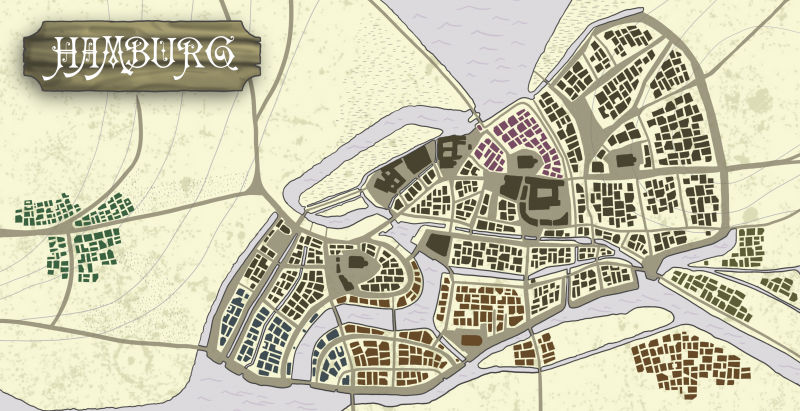
\includegraphics[scale=0.7]{./images/Karte.png}
		\caption{Stadkarte von Hamburg, anno 1350}
    \label{fig:Karte}
	\end{center}
\end{figure}


\subsection{Das Gespräch mit dem Rat}

Also Ihr euch also unterhaltet öffnet sich plötzlich die Holztür und ein junger Ratsdiener bittet euch vor den Rat zu treten.

\red{\textbf{Szene}}: Vor dem Hamburger Rat

\textbf{Raumbeschreibung}: Ihr tretet in einen großen Raum ein, der von einer U-förmigen Tischreihe dominiert werden, an dem 18 Männer in erhöhter Position sitzen. Auch wenn der Raum sonst nur spärlich eingerichtet ist, ist offensichtlich dass sich hier sonst niemand aufhält, der wenig Geld hat. Aus den Wänden sind kunstvoll Löwenköpfe und andere Muster herausgearbeitet. Eine Wand ist von hohen Fenstern gesäumt, die den Raum hell erleuchten.

Im Hintergrund huschen Ratsdiener mit Papieren umher oder gehen anderen Aufgaben nach.

\red{\textbf{Info}: Die 18 Männer setzen sich aus neun Rechtskundigen, sieben Kaufleuten und zwei Vertretern der Kirche zusammen.}

\red{\textbf{Interaktion}}:

Vorsitzender des Rates:
\gqm{\textit{Der Hamburger Rat dankt euch für euer Erscheinen. Bevor wir uns jedoch mit den euch betrauten Aufträgen befassen werden, sagt, was wisst ihr über die Pestilenz?}}

\red{\textbf{Probe auf Gesellschaft/Wissen o.Ä}: Menschen die von der Pestilenz befallen sind leiden unter Schwindelgefühlen und Schüttelfrost. Auch klagen manche über starke Kopfschmerzen und erbrechen sich häufig. Ein hohes Fieber sowie schwarze Pestbeulen an den Lymphknoten treten im Verlaufe der Krankheit auf und sind für den Patienten meist ein sicheres Todeszeichen.}

\red{\textbf{kritischer Erfolg/Probe auf Medizin}: Manche Heiler berichten, dass sie die Pestbeulen aufschneiden und vom darin enthaltenden Eiter reinigen. Wird anschließend das Fieber eines Kranken behandelt konnte mancher Totgeglaubte wieder von der Pest geheilt werden.}

Vorsitzender des Rates:
\gqm{\textit{}}


\section{\textbf{Kapitel 2 - Im Sitz des Beirats}}

%!TEX root = ../main.tex

\red{\textbf{Szene}}:

Nachdem ihr aus dem Rat entlassen wurdet macht ihr euch also auf den Weg zum Sitz des Beirats. In der unmittelbaren Umgebung des Ratshauses spürt man den Aufstieg Hamburgs als Handelsmetropole am deutlichsten. Ihr schlendert durch breite Straßen die von hohen Häusern gesäumt werden. Dienstboten eilen über den Pflasterstein und auch sonst herrscht geschäftiges treiben, als ihr unweit der St. Michaelis Kirche vor eine Kapelle tretet, die euch der Rat als eure Operationszentrale genannt hat

\textbf{Raumbeschreibung}: Als ihr an der kleinen Kapelle ankommt, erkennt ihr, dass es sich dabei um ein durchaus anschauliches Gebäude handelt, dass erst kürzlich einen neuen Anstrich mit weißer Farbe erhalten hat. Im Inneren stehen allerhand Tische und Stühle herum. Außerdem gibt es Schlafmöglichkeiten und so ziemlich alles, was man zum Leben so gebrauchen kann. Selbst ausgewählte Speisen stehen bereits zum Verzehr bereit.

\textbf{Ereignis}: Die Gruppe kann sich erst mal unterhalten. Ihr Gespräch wird allerdings von einem Klopfen unterbrochen ...

\begin{tcolorbox}
  Wurf: Wer oder was unterbricht das Gespräch unserer Gruppe?
  Das Militär (1 bis 33) (gehe zu \ref{militär}) \\
  Der Tod (34 bis 66) (gehe zu \ref{tot}) \\
  Ein Kind (67 bis 99) \ref{kind} \\
  Bei 100: würfle erneut.
\end{tcolorbox}

\section{Der militärische Besuch}
\label{militär}

\red{\textbf{Szene}}:

General zur Brügge steht davor und bittet um Einlass.

Gespräch mit Brügge: Dieser berichtet ihnen in vehementem Ton, dass die ganze Krise ein Werk der Dithmarscher sei. Diese hätten sich jahrelang an Hamburgs Handelsschiffen gütlich getan. Nun, da es einen Vertrag gibt, der das verhindert, versuchen einige von ihnen die Stadt zu schwächen, um davon zu profitieren oder sie gar ganz an sich zu reißen. Die Dithmarscher operieren von ihrem Versteck aus, das sich in einer Hafenkaschemme namens „Beim Gelockten Hund“ befinden soll. Ein gewisser Gorich leite das Ganze. Dort sollten sie mit ihren Recherchen beginnen.

Interaktionen:

Probe auf Menschenkenntnis:

General zur Brügge sagt schon die Wahrheit, aber seine Perspektive könnte durchaus verzerrt beziehungsweise einseitig sein.
Die Charaktere können sich aber sicher sein, dass er nicht lügt, zumindest seiner Auffassung nach nicht.

Ab hier können die Spieler frei entscheiden, wohin sie gehen wollen! Nach Ablauf der Frist von vier Tagen müssen sie beim Hamburger Rat vorsprechen. Bis dahin müssen sie sich auf eine Handlungsempfehlung festgelegt haben!


Option 2 – Der Tod
\red{\textbf{Szene}}:

Ereignis: Während sich die Gruppe noch unterhält, hören die Charaktere plötzlich ein lautes Klopfen an der Tür.

Davor steht der Totensammler Hanno. Er fragt, ob es Tote gäbe, die abzuholen seien, und ob im Haus bereits die Pest wüte.

Gespräch mit Hanno: Im Armenviertel sei es am Schlimmsten. Die Leichen könne er kaum mehr entsorgen. Man müsse kreativ werden.

Gegen Bestechung verrät er, dass er jemandem Leichen verkaufe. Dazu müsse er sie allerdings recht weit fortbringen, nämlich in einen kleinen Ort namens Eeksdurf vor den Toren der Stadt. Dort hinterlege er die leblosen Körper in einem Lagerhaus, wo bereits seine Bezahlung auf ihn warte. Die Absprache habe er dereinst mit einer jungen rothaarigen Frau getroffen.

Sie habe ihn angesprochen, nachdem sie ihn beim Abholen von Leichen im Dorf sah...


Ab hier können die Spieler frei entscheiden, wohin sie gehen wollen! Nach Ablauf der Frist von vier Tagen müssen sie beim Hamburger Rat vorsprechen. Bis dahin müssen sie sich auf eine Handlungsempfehlung festgelegt haben!


Option 3 – Ein Kind
\red{\textbf{Szene}}:

Ereignis: Es klopft plötzlich an der Tür und davor steht ein Kind zusammen mit seiner stark vermummten Mutter.

Gespräch mit der Mutter und dem Kind: Sie kämen aus dem Armenviertel Hammerbrook und seien auf der Suche nach der St. Petri-Kirche. Sie soll ein Zufluchtsort für gesunde und sündenfreie Menschen sein. Niemand werde dort krank! Für sie sei es zu spät, hustet die Frau, aber ihr kleines Kind, das sei noch zu retten. Sie wissen das alles von einem Mann, der im Armenviertel nach den Leuten sehe. Er werde nicht krank, egal was er tue ... Er habe sie losgeschickt. Sie wüssten gern den Weg.

Die Gruppe kann eine Beschreibung von Didrich von Sinnfeld erhalten. Außerdem geben ihnen die beiden auf Nachfrage den Tipp, einmal beim Lumpensammler im Armenviertel vorbeizuschauen.


Ab hier können die Spieler frei entscheiden, wohin sie gehen wollen! Nach Ablauf der Frist von vier Tagen müssen sie beim Hamburger Rat vorsprechen. Bis dahin müssen sie sich auf eine Handlungsempfehlung festgelegt haben!


\section{\textbf{Kapitel 3 - Am Hafen}}
\label{Hafen}
%!TEX root = ../main.tex

\red{\textbf{Szene}}:

Nach einem kurzen Fußmarsch steht ihr nun also inmitten des Hafens. Es herrscht geschäftiges Treiben. Allerlei Matrosen (\blue{\ref{Matrosen}}) und Hafenarbeiter (\blue{\ref{Hafenarbeiter}}) gehen ihren Aufgaben nach. An den Kais stehen einige Aufseher (\blue{\ref{Aufseher}}) und löschen die Ladungen der vor Anker liegenden Handelsschiffen.

\textbf{Ortsbeschreibung}: Allerhand Gesindel und unzählige Hafenarbeiter treiben sich herum. Prostituierte (\blue{\ref{Prostituierte}}) bieten ihre Dienste an, und Kinder betteln um ein wenig Brot. Hin und wieder sieht man Menschen, die sich vermummen oder gar ihr ganzes Gesicht hinter Tüchern verbergen.

\red{\textbf{Interaktionen}}:

Die Gruppe kann sich nun zum „Gelockten Hund“ aufmachen oder sich zunächst ein wenig umsehen. An den Docks treffen sie auf allerhand Charaktere, die ihnen etwas zum Hafen erzählen können.
Diese werden ihnen erzählen, dass immer mehr Arbeiter ausfallen, die mit der Lagerung von Lebensmitteln und anderen verderblichen Waren zu tun haben.

\subsection{Vor dem \gqm{Gelockte Hund}}
\label{vorhund}

\red{\textbf{Szene}}:

Ihr haltet vor einem kleinen Wirtshaus dessen besten Tage bereits weit in der Vergangenheit liegen. Es sieht - wie seine Kundschaft - ein wenig heruntergekommen aus. Vor der Türe des Gebäudes halten sich drei finstere Gestalten, bei denen es sich wohl um Seeräuber handelt, auf.

Ereignis: Schon vor der Tür wird die Gruppe unangenehm begrüßt. Die Seeräuber behaupten es würde Eintritt kosten, in den Laden zu kommen.

Es gibt nun verschiedene Möglichkeiten an den Seeräubern vorbei in das Gasthaus zu gelangen:

\begin{itemize}
  \item \red{\textbf{Probe auf Menschenkenntnis (erleichtert):} Dass der Eintritt etwas kostet, ist eine Lüge.} \\
  \item \textbf{\red{Kampf:}} Betrunkener Pirat \\
\begin{center}
  \begin{tabular}{cc}
  \toprule
  Fähigkeit & Punkte \\
  \midrule
  Leben & 80 \\
  Fäuste & 70 \\
  Schaden & 15 \\
  Parieren & 5 \\
  \bottomrule
\end{tabular}

\end{center}

Werden die Piraten besiegt können die Spieler ein verziertes Kreuz aus Silber in der Tasche eines Piraten finden.

\red{\textbf{Probe auf christliche Kultur o.ä.}: Es ist ein Kreuz, wie es sonst nur Priester tragen würden.
Auf der Rückseite ist Apostel Petrus eingraviert.}
\end{itemize}

\subsection{Im \gqm{Gelockten Hund}}
\label{imhund}

\red{\textbf{Szene}}:

Der Eindruck, dass es sich hier um eine finstere Absteige handelt bestätigt sich, als ihr eintretet. Auch das Innere dementsprechend heruntergekommen aus. Der Großteil des Publikums ist Gesindel, das Fremden gegenüber nicht sonderlich wohlgesonnen sein dürfte.

\textbf{Raumbeschreibung}: Es herrscht ausgelassene Stimmung. In der Kaschemme selbst ist erst mal aber nichts besonders ungewöhnlich.

\red{\textbf{Interaktionen}}:

Die Charaktere können sich umhören, ob jemand Gorich kennt. Sollten sie nach ihm fragen wird niemand bis auf den Wirt Gert (\blue{\ref{Gert}}) ihnen antworten.

Gert: \gqm{\textit{Edle Herren, ich würde euch gerne Auskunft geben, doch seht was hier los ist! Heute morgen ist meine Wirtin nicht zur Arbeit erschienen. Auch meine Frau, die das Essen zubereitete ist letzte Woche der Pest zum Opfer gefallen. Wenn ihr mir... ein wenig unter die Arme greifen könntet? Danach werde ich euch freilich gerne helfen!}}

Entscheidet sich die Gruppe dem Wirt Gert zu helfen, dann muss sie ihn nun bei Aufgaben in der Kneipe unterstützen. Diese Aufgaben sind:

\begin{itemize}
  \item Eintopf kochen (Probe auf Kochen o.Ä)
  \item Gäste bedienen (Probe auf Menschenkenntnis (erleichtert))
  \item Einen Streit schlichten (Probe auf Beruhigen o.Ä)
  \item Ein wenig Musizieren (Probe auf passendes Talent)
\end{itemize}

Für einen Erfolg müssen mindestens zwei der Aufgaben erfolgreich bestanden werden. Sind mehr Aufgaben erledigt kann der Wirt je nach Ermessen des Spielleiters den Abenteurern einen Schilling für ihre Dienste geben.

Schafft die Gruppe es nicht zwei der vier Aufgaben zu bewältigen gibt Gorich sich nicht zu erkennen. Er kann nur noch mit Gewalt oder Tricks dazu gebracht werden, sich zu offenbaren. Dies ist aber stark erschwert.

\red{\textbf{Szene}}:

Ein großer, bärbeißiger Mann mit schmalem Gesicht und noch schmaleren Augen tritt an euch heran. Er stellt sich als Gorich (\blue{\ref{Gorich}}) vor. Er erzählt den Abenteurern er und seine Leute haben nichts mit der ganzen Sache zu tun. Er zeigt der Gruppe sogar, dass seine eigenen Kinder im Hinterzimmer liegen... krank. Sie hatten schon früh von der Seuche gehört und auch erfahren, dass es irgendwas mit Lebensmitteln zu tun haben könnte. Denn es waren zuallererst die Bauern und Karrenlenker krank geworden, die im Umland lebten. Also kaufte er all seine Nahrung nur noch aus Einfuhr. Das schien aber auch nichts zu helfen. Denn seine Frau ist bereits gestorben, und auch seinen Kindern gehe es immer schlechter. Ein gewisser Hagen habe es ihm verkauft. Dieser lebe in Hammerbrook, direkt vor den Toren der Stadt. Gekauft habe er die Güter direkt bei einem Lagerarbeiter. Er wisse, dass auch andere, die bei ihm gekauft haben, krank wurden.

Bevor die Abenteurer aufbrechen wird Gorich sie bitten seine Kinder und ihn nicht zu verraten. Das würde den Untergang seines Geschäfts bedeuten, und dann könne er sich erst recht nicht mehr um sie kümmern.

\red{\textbf{Interaktionen}}:

\red{\textbf{Probe auf Menschenkenntnis}: Gorich scheint die Wahrheit zu sagen.}

\purple{\textbf{Pestilenz}: Jeder, der sich den Kindern von Gorich nähert, erhält Pestilenz +2.}

\green{\textbf{Moral}: Was tut die Gruppe also mit Gorich und seinen Kinder?}

Ende des relevanten Hafen-Plots. Weiter mit:

Eeksdurf (gehe zu \blue{\ref{Eeksdurf}}) \\
Hammerbrook (gehe zu \blue{\ref{Hammerbrook}}) \\
Die Kirche St. Petri (gehe zu \blue{\ref{Petri}}) \\
Der Nikolaifleet (gehe zu \blue{\ref{Fleet}}) \\


\section{\textbf{Kapitel 4 - Eeksdurf}}
\label{xd}
%!TEX root = ../main.tex

\subsection*{Der Weg nach Eeksdurf}
\label{nachxd}

Ihr macht euch also auf den Weg nach Eeksdurf. Schon bald drängen sich die Häuser weniger dicht und ihr verlasst Hamburg in Richtung Westen. Größtenteils verläuft der Weg aus gestampfter Erde gerade durch die Felder, an ein paar Stellen teilt sich der Weg und ihr folgt den Wegweisern nach Eeksdurf. So seid ihr also etwa eine halbe Stunde unterwegs als ihr plötzlich am Wegesrand etwas bemerkt.

\red{\textbf{Szene}}:

Im Straßengraben liegt umgekippt ein Karren. Wollen die Spieler die Szene genauer untersuchen entdecken sie, dass die Speichen der Räder gebrochen sind. Außerdem liegen im Straßengraben drei Leichen. Einer der Toten trägt ein Priestergewand und liegt mit durchgeschnittener Kehle dahingestreckt.

\red{\textbf{Probe auf Medizin o.ä.(erleichtert)}: Die anderen beiden Toten wurden durch Stichwunden in den Oberkörper getötet}

Es scheint sich um einen Raubüberfall zu handeln. Wertsachen finden sich hier keine, auch Teile ihrer Kleidung wurden den Leichen vom Leib gerissen.

\red{\textbf{Probe auf christliche Kultur o.ä. (erleichtert)}: Selbst das Kreuz, welches der Priester mit Sicherheit um den Hals trug, ist verschwunden.}

\red{\textbf{Information für den Spielleiter}: Das Kreuz kann die Gruppe an einem betrunkenen Piraten vor dem "Gelockten Hund" im Hafen finden.}

Ihr findet sonst keinen Hinweis darauf, wer die Verstorbenen sein könnte. Allerdings entdeckt ihr einige Pergamente, die in lateinischer Schrift verfasst sind.

\red{\textbf{Probe auf Latein o.ö}: Die Pergamente handeln von schwarzer Magie und anderem Volksglauben.}

Außerdem finden die Spieler bei genauerem Hinsehen in der Brusttasche des Priesters ein Brief von einem Wolfgang (\blue{\ref{Wolfgang}}) aus Eeksdurf, in dem dieser die Kirche um sofortigen Beistand in einer dringenden Sache bittet.

Ein gutes Dutzend Fußspuren führt weiter in Richtung Eeksdurf, aber auch genügend in Richtung Hamburg. Schwer zu sagen, ob sie von den Tätern oder anderen Reisenden stammen. Aber in jedem Falle sind die Spuren am Ort der Tat nicht älter als eine Stunde. Mehr ist hier nicht zu finden.

\subsection*{Ankunft in Eeksdurf}
\label{inxd}

\red{\textbf{Szene}}:

So macht ihr euch also weiter auf den Weg nach Eeksdurf. Nach einer weiteren halben Stunde seht ihr wie zwischen Bäumen die ersten Häuser des kleinen Dorfes hervortreten. Ihr folgt dem Weg und steht bald in dem kleinen Örtchen auf einer menschenleeren Straße. Durch den alltäglichen Klatsch und Tratsch wisst ihr, dass die meisten Einwohner hier einfache Handwerker und Bauern sind. Vom sonst so geschäftigen Treiben ist nun nichts mehr zu spüren, es ist alles verlassen. Türen und Fenster sind verrammelt.

Klopfen die Spieler an eine der Türen, dann antwortet man ihnen, wenn sie passend würfeln.

\begin{tcolorbox}
  Wurf: Wird ihnen auf das Klopfen geantwortet? \\
  0 bis 49: Ihnen wird geantwortet. \\
  50 bis 99: Ihr Klopfen bleibt unbeantwortet.\\
\end{tcolorbox}

Sollte einer der Dorfbewohner mit ihnen sprechen macht er einen verängstigten Eindruck. Wo die anderen alle seien wisse er nicht.

\red{\textbf{Probe auf Menschenkenntnis}: Das er nicht wisse wo alle seien ist eine Lüge.}

Fragen die Spieler nach einer rothaarigen Frau erzählt man ihnen von Ruth (\blue{\ref{Ruth}}), der Tochter der Kräutersammlerin Ottilde (\blue{\ref{Ottilde}}). Diese wohne gleich die Straße runter am Dorfesrand in einer kleinen verfallenen Hütte. Wenn man der Straße folge könne man es nicht verfehlen.

\red{\textbf{Probe auf Menschenkenntnis}: Auch die Wegweisung ist eine Lüge.}

Folgen die Spieler diesem Weg gelangen sie bald an den Dorfesrand, dort ist nirgends ein Haus zu sehen, das auf die Beschreibung des Dorfbewohners passt. Jedoch hören die Abenteurer ein Geräusch...

\begin{tcolorbox}
  Wurf: Was hört die Gruppe? \\
  1 bis 50: Sie hören aufgebrachte Stimmen. (gehe zu \blue{\ref{mob}})\\
  51 bis 100: Sie hören ein Knacken und Rauschen. (gehe zu \blue{\ref{feuer}})\\
\end{tcolorbox}

\subsubsection*{Option 1 - Der wütende Mob}
\label{mob}

\red{\textbf{Szene}}:

Ihr folgt den Geräuschen und gelangt an eine kleine Hütte vor dem Waldrand. Die Hütte macht einen verfallenen Eindruck, scheint aber noch bewohnt zu sein. Vor der Haustüre stehen wütend grölende Menschen und schwingen Mistforken, während eine alte, merkwürdig gekleidete Dame vor der Hütte versucht sie zu besänftigen.
Aus den aufgebrachten Wortgefechten lässt sich schließen, dass es sich bei der Dame um die Kräuterfrau Ottilde handelt.

Der Rädelsführer des Mobs ist ein Bauer namens Wolfgang (\blue{\ref{Wolfgang}}). Dieser fordert vehement, dass Ruth aus dem Haus herauskommt. Sie sei an dem Unglück Schuld! Schwarze Magie habe sie angewandt und nicht mal die Kirche wolle den Bewohnern mehr helfen, obwohl man mit einem Brief um Hilfe gebeten hatte!

\red{\textbf{Interaktionen}}:

Die Gruppe sollte versuchen den wütenden Mob zu beruhigen. Im Gespräch werden die Leute im Mob sich immer wieder auf vier Argumente berufen:

\begin{itemize}
  \item Ruth soll wiederholt dabei gesehen worden sein, wie sie nachts tote Körper in die große Scheune gebracht habe.
  \item Ruth habe den Brief an die Kirche, welchen sie dem Totensammler mitgeben sollte, nie übergeben.
  \item Ruth habe die Pest gebracht. Sie war in Hamburg gewesen, um Korn zu kaufen.
  \item Kaum war sie zurück, brach die Krankheit aus! Zu diesem Zeitpunkt sei noch nirgends sonst in der Gegend jemand erkrankt!
\end{itemize}

\red{\textbf{Probe auf Beruhigen}}:

\begin{itemize}
  \item Erfolg \\
  Schaffen Sie es den Mob zu beruhigen, dann zieht sich der Mob zurück und sie können mit Ottilde in Ruhe das Haus betreten. Dort treffen sie auch auf Ruth, die verängstigt in einer Ecke sitzt.
  \item Misserfolg \\
  Schaffen sie es nicht den Mob zu beruhigen, dann bricht dieser in das Haus ein. Wollen die Abenteurer den Mob hindern kommt es zum Kampf (\blue{\ref{kampf}}) mit Bauern. Im Haus fehlt jedenfalls so oder so jede Spur von Ruth. Ottilde ist dankbar für ihre Hilfe und verrät der Gruppe, dass Ruth sich in der großen Scheune verstecke.
\end{itemize}

Ruth wird der Gruppe kleinlaut erzählen, dass sie nichts gemacht habe und nicht wisse warum die Bauern so aufgebracht seien

\red{\textbf{Probe auf Menschenkenntnis}}:

Ruth lügt. Hakt die Gruppe nach, dann erzählt sie, ihnen die gesamte Geschichte. \\
Sie habe direkt am Nikolaifleet Korn holen wollen. Da sei es am günstigsten, habe man ihr gesagt. Als sie dort ankam, sei es bereits spät gewesen. Sie habe am Lagerhaus, das man ihr beschrieben hatte, angeklopft, allerdings ohne Erfolg. Also habe sie durchs Fenster geschaut und einen Mann erblickt, der sich über etwas gebeugt habe. Er soll eine Art Vogel-Maske und einen weiten Mantel getragen haben. Ruth sagt, sie habe Angst gehabt und habe davonlaufen wollen. Sie sei auf dem Schnee ausgerutscht und habe das Gleichgewicht verloren. Dabei sei mit dem Kopf aufgeschlagen und im Lagerhaus wieder zu sich gekommen. Der Mann habe sich ihr dann als Didrich vorgestellt. Er forsche an der Pestilenz, habe er erklärt. Nur darum sei er so gekleidet und habe sich an der Leiche zu schaffen gemacht. Ruth habe ihm dann erzählt, dass in Eeksdurf zwar niemand krank sei, aber dass der Totensammler regelmäßig mit den Leichen durch ihr Dorf fahre, um diese tief im Eekshult zu verscharren. Daraufhin habe Didrich ihr einen Handel vorgeschlagen, und... naja... Ruth habe angenommen. \gqm{\textit{Wieso auch nicht. Die sind schließlich tot und ich arm. Eins davon kann man wenigstens noch ändern.}}
Die Leichen habe sie also von da an immer in ein kleines Lagerhaus im Armenviertel Hammerbrook gebracht. Dort habe auch ihr Geld gelegen...

Sollte die Gruppe nachfragen, kann Ruth ihnen genau sagen, in welchem Lagerhaus sie die Leichen ablegt.

\subsubsection*{Option 2 – Ein großes Feuer}
\label{feuer}

\red{\textbf{Szene}}:

Ihr folgt den Geräuschen und gelangt an eine kleine Hütte vor dem Waldrand. Die Hütte macht einen verfallenen Eindruck, scheint aber noch bewohnt zu sein. Es ist weit und breit niemand zu sehen, vor der offenen Tür der Hütte seht ihr jedoch ein gewaltiges Feuer. Im Feuer zeichnen sich die verkohlten Überreste zweier Menschen ab.

Die Gruppe kann wenn gewünscht die Hütte betreten.

\textbf{Raumbeschreibung}: Das Innere der Hütte macht genauso wenig her wie die Fassade vermuten lässt. In einer Ecke des einzigen Raumes ist Stroh auf dem Boden ausgebettet. Ein morscher Holztisch und zwei Stühle stehen in der anderen Ecke. Das einzige herausstechende im Raum ist ein Regal, dass eine ganze Wand einnimmt, und auf dem getrocknete Kräuter säuberlich aufgereiht sind.

Bei genauerem Hinsehen findet die Gruppe ein Blatt Pergament, auf dem eine Art Wegbeschreibung gekritzelt zu sein scheint - nur sehr grob. Der Weg führt zu einem Ort im Armenviertel Hammerbrook, mehr lässt die Karte nicht erkennen. Außerdem finden die Abenteurer Geld. Etwas mehr Geld als jemand der hier lebt besitzen sollte.

Beim Verlassen der Hütte trifft die Gruppe auf Wolfgang (\blue{\ref{Wolfgang}}) und Hermann (\blue{\ref{Hermann}}). Diese werfen ihnen umgehend vor, mit der bösen Zauberin im Bunde zu sein und werden sie angreifen (gehe zu \blue{\ref{kampf}}) falls die Gruppe nicht schafft die beiden zu beruhigen.

\red{\textbf{Probe auf Beruhigen o.ä}: Die Bauern erzählen, weshalb sie Otthilde und Ruth verbrannt haben}

\begin{itemize}
  \item Ruth soll wiederholt dabei gesehen worden sein, wie sie nachts tote Körper in die große Scheune gebracht habe.
  \item Ruth habe den Brief an die Kirche, welchen sie dem Totensammler mitgeben sollte, nie übergeben.
  \item Ruth habe die Pest gebracht. Sie war in Hamburg gewesen, um Korn zu kaufen.
  \item Kaum war sie zurück, brach die Krankheit aus! Zu diesem Zeitpunkt sei noch nirgends sonst in der Gegend jemand erkrankt!
\end{itemize}

\subsubsection*{Kampf gegen die Bauern}
\label{kampf}

\begin{center}
  \begin{tabular}{lcc}

    \toprule
    Fähigkeit & \textbf{Wolfgang} & \textbf{Hermann} \\
    \midrule
    Leben & 70 & 70 \\
    Waffe & Fäuste (70) & Mistgabel (70) \\
    Schaden & 15 & 40 \\
    Parieren & 5 & 30 \\
    \bottomrule
  \end{tabular}
\end{center}



\violet{\textbf{Moral}: Wie reagiert unsere Gruppe auf die Situation in Eeksdurf?}

Ende des relevanten Eeksdurf-Plots.

Hafen (gehe zu \blue{\ref{Hafen}}) \\
Hammerbrook (gehe zu \blue{\ref{arm}}) \\
Die Kirche St. Petri (gehe zu \blue{\ref{Petri}}) \\
Der Nikolaifleet (gehe zu \blue{\ref{Fleet}}) \\


\section{\textbf{Kapitel 5 - Hammerbrook}}
\label{arm}
%!TEX root = ../main.tex

\brown{\textbf{Pestilenz}: Jeder, der das Armenviertel betritt, erhält +1 Pestilenz.}

\red{\textbf{Szene}}:

Ihr kommt also in Hammerbrook an, einem der Stadtviertel in denen sich die Ärmsten der Stadt zusammenpferchen in der Hoffnung vom Reichtum zu profitieren den der Handel in Hamburgs Kassen spült. Dicht gedrängt leben hier Hafenarbeiter, einfache Leute und anderes Gesindel in ärmlichen Hütten und Häusern. Man merkt, dass hier andere Regeln zu gelten scheinen als im Rest der Stadt, die Straßen sind gesäumt von Toten und Kranken, und in kaum einem Haus brennt Licht. Der Tod geht um, und tagtäglich rechnen hier viele mit dem schlimmsten.

\subsection{Auf den Straßen}
\label{strasse}

\red{\textbf{Szene}}:

Die Straßen sind verschneit und verlassen. Nur vereinzelt ziehen vermummte Gestalten umher und werfen unserer Gruppe argwöhnische Blicke zu. Ihr scheint hier nicht willkommen zu sein.

\red{\textbf{Information für den Spielleiter}: Sollte einer der Spieler in auffallend feinen Kleidern durch das Armenviertel wandern wird die Gruppe später überfallen. (gehe zu} \blue{\ref{kampf2}}\red{).}

Plötlich kommen mehrere verhärmte Kinder unter lautem Geschrei auf euch zu. Sie haben einen unförmigen Lederklumpen dabei und scheinen ganz offensichtlich Fußball zu spielen. Als sie auf eurer Höhe sind rempeln einige der größeren Kinder euch an und murmeln eine Entschuldigung, bevor sie wieder in einer Seitengasse verschwinden.

\red{\textbf{Probe auf Gassenwissen o.ä.}: Alle würfeln eine Probe. Wer diese erfolgreich besteht bemerkt, dass ihm ein Gegenstand geklaut wurde.}

Während die Spieler das bemerken (oder auch nicht!) biegen die Kinder gerade aus ihrem Sichtfeld in eine kleine Seitengasse ein. Die Spieler können die Kinder jedoch noch versuchen mit einer Probe auf Rennen (um 10 erschwert) die Kinder zu verfolgen.

\begin{itemize}
  \item Erfolg: Holen sie die Kinder ein (gehe zu \blue{\ref{eingeholt}}).
  \item Misserfolg: Die Gegenstände sind verloren (gehe zu \blue{\ref{neingeholt}})
\end{itemize}

\subsection{Option 1 - Beim Lumpensammler}
\label{eingeholt}

\red{\textbf{Szene}}:

Ihr verfolgt also die Kinder bis diese die Tür zu einem Laden aufstoßen und darin verschwinden. Wenige Momente später betretet auch ihr außer Atem den Laden. Von den Kindern ist keine Spur zu sehen. Jedoch begrüßt der Lumpensammler Luis (\blue{\ref{Luis}}) überschwänglich die neue \gqm{Kundschaft}.

Auf Nachfrage stellt sich heraus, dass der Lumpensammler die Gegenstände der Spieler hat, aber nicht ohne weiteres herausgeben will. Nun hat die Gruppe folgende Optionen:

\begin{itemize}
  \item Probe auf Einschüchtern, um 30 erschwert (gehe zu \blue{\ref{fertig}})
  \item Die Gruppe geht wieder (gehe zu \blue{\ref{neingeholt}})
  \item Der Lumpensammler möchte mit den Spielern wetten (gehe zu \blue{\ref{wette}})
\end{itemize}

\subsubsection{Das Rätsel}
\label{wette}

Lumpensammler: \gqm{\textit{Ich hab es! Wir schließen eine Wette ab, ich stelle euch ein Rätsel das es zu lösen gilt. Wenn ihr es löst gebe ich euch eure Sachen wieder, schließlich können so piekfeine Schnösel wie ihr es seid bestimmt gut ein Rätsel lösen?}}

Voller Hochmut und Vorfreude trägt der Lumpensammler das Rätsel vor:

Lumpensammler: \gqm{\textit{Einst wurde ein Pirat gefasst der dem König sein Gold gestohlen hatte. Der König tobte und verlangte, dass der Pirat unverzüglich am Galgen aufgeknüpft werde. Es war aber üblich, den zum Tode verurteilten Dieben eine letzte Chance zu geben und Gott über sie richten zu lassen. Daher mussten sie aus einem schwarzen Säckchen einen Stein ziehen. Im Säckchen befanden sich immer genau ein weißer und ein schwarzer Stein. Zog der Dieb den weißen Stein, wurde ihm die Freiheit geschenkt. Zog er hingegen den schwarzen Stein, so baumelte er.  Eines Tages kam nun jener Pirat der einst das Gold des Königs geraubt hatte vor den Scharfrichter und wartete auf sein Gottesurteil.}}

Lumpensammler: \gqm{\textit{Der König aber wollte sichergehen, dass der Halunke hängt und hat dem Henker am Abend zuvor im Heimlichen befohlen zwei schwarze Steine in das Säckchen zu legen.
So ging der König am nächsten Tage also voller Zuversicht also zum Richtplatz, wo überall weiße und schwarze Steine herumlagen. Als es Zeit wurde für den Verurteilten sein Urteil zu erhalten bückte sich der Henker und nahm zwei schwarze Steine vom Boden auf, die er im Säckchen ablegte. Der Pirat sah dies jedoch und wusste somit, dass er kein gerechtes Urteil erhalten würde. Er glaubte die Schlinge schon um seinen Hals als ihm die rettende Idee kam. \\
Er zog einmal und musste freigelassen werden. \\ Was war es, dass dem Piraten das Leben rettete?}}

\begin{itemize}
  \item Erfolg: Die Lösung des Rätsels besteht darin, dass der Dieb einen Stein zieht und ihn sogleich wegwirft. Da der verbleibende Stein im Sack schwarz ist, muss der gezogene Stein scheinbar weiß gewesen sein. Beantwortet die
  \item Misserfolg: Können sie das Rätsel nicht lösen oder liegen falsch wird der Lumpensammler ihnen ihre Gegenstände nicht zurückgeben, er genießt seinen Triumph viel zu sehr!
\end{itemize}

\subsubsection{Abschließen der Aufgabe}
\label{fertig}

Ungeachtet der vorigen Ereignisse wird der Lumpensammler ihnen erzählen, dass sie nicht die ersten wohlbetuchten Personen sind, die in den letzten Tagen in seinem Laden waren. Es ist noch nicht allzu lange her, da sei einer in einem ganz komischen Aufzug hier hereingeschneit. Er habe nach abstrusen Pflanzen gefragt. Chillies und Zitronen seien darunter gewesen. Als ob man sowas hier bekomme. Außerdem habe er noch einen Blasebalg gewollt und etwas grobes Leinen, Lumpen und Teer. Komischer Typ.

Er kann den Abenteurern jedoch die grobe Richtung beschreiben in die der Kunde verschwunden ist. Nachdem er ihnen das erzählt hat drängt Luis die Gruppe zu gehen, er hat noch andere Kundschaft um die er sich kümmern muss. Wieder auf der Straße stehend können die Spieler nach der Person fragen die der Lumpensammler ihnen beschrieben hat oder dem vorgeschlagenen Weg folgen. Nach einem kurzen Fußmarsch kommen sie dann an einem Lagerhaus an (gehe zu \blue{\ref{Lagerhaus}})

\subsection{Das Treffen mit Sigrun}
\label{neingeholt}

\red{\textbf{Szene}}:

Ihr probiert noch den Kindern nachzueilen, doch als ihr um die Ecke biegt hinter der ihr sie eben noch verschwinden sehen habt ist keine Spur mehr zu finden, sie scheinen sich in Luft aufgelöst zu haben.

Jedoch schaut euch eine dicklichere Frau verwundert an.

Frau: \gqm{\textit{Ihr wurdet wohl von den Kindern hier ausgeraubt? Findet euch lieber schnell mit dem Verlust ab, in den Gassen hier habt ihr keine Chance sie noch irgendwo aufzufinden.}}

Im weiteren Verlauf des Gesprächs stellt sie sich als die Bäckerin Sigrun (\blue{\ref{Sigrun}}) vor. Sie folgt dem Ruf von Pater Salus und ist gerade auf dem Weg nach St. Petri. Dort sind unzählige Menschen und keiner von ihnen ist krank. Ein sicherer Aufenthalt, so scheint es. Allerdings müsse sie erst in Erfahrung bringen, ob auch ihre Kinder dort Willkommen seien, da sie mit Fieber zu Hause im Bett liegen. Sigrun bittet die Gruppe, bei ihr zu Hause vorbeizuschauen und nach den Kindern zu sehen während sie weg ist.

\violet{\textbf{Moral}: Wie wird die Gruppe mit der Bitte von Sigrun umgehen?}

\begin{itemize}
  \item Die Gruppe hilft den Kindern nicht, Sigrun zieht niedergeschlagen davon, und die Gruppe bleibt auf sich gestellt.
  \item Sie helfen den Kindern, Sigrun weist ihnen den Weg zu ihrem Haus und verrät, wo der Zweitschlüssel hinterlegt ist.
\end{itemize}

\subsubsection{Bei Sigrun Zuhause}

\red{\textbf{Szene}}:

Nach einem kurzen Fußmarsch steht ihr vor Sigruns Haus. Vor der Türe des Hauses steht ein Gestell, auf dem Brote zum Verkauf angeboten werden können, momentan ist es jedoch leer. Ansonsten gibt es nicht viel zu sehen. Ein unangenehmer Geruch liegt in der Luft. Öffnen die Spieler die Türe wird der Geruch stärker.

\brown{\textbf{Pestilenz}: Alle die das Haus betreten erhalten +2 Pestilenz.}

In einem der Zimmer findet ihr zwei schweissnasse Kinder zugedeckt in einem Bett liegen. Eines der Kinder weint lautstark, das andere regt sich nicht.

\red{\textbf{Probe auf Medizin o.ä}: Den Kindern ist nicht mehr zu helfen, zumindest nicht mit euren Fähigkeiten.}

\brown{\textbf{Pestilenz}: Kümmern sich die Spieler weiter um die Kinder erhalten sie +1 Pestilenz.}

\subsubsection{Das Treffen mit Hagen}
\label{klopf}

\red{\textbf{Szene}:}

Plötzlich klopft es an der Türe. Ein blonder, kräftig gebauter staht auf der Straße und fragt die Gruppe wo Sigrun sei und was sie hier zu suchen hätten. Nach einer Erklärung stellt er sich als Hagen (\blue{\ref{Hagen}}) vor und läd sie zu sich nach Hause ein, er habe ihnen etwas spannendes zu erzählen! Folgt ihm die Gruppe gelangen sie nebenan zu Hagens Haus.

\textbf{Raumbeschreibung}: Hagens Haus ist aufgeräumt. Nirgendwo liegen Waren oder ähnliches herum und auch sonst ist es nur kärglich eingerichtet Einige Kerzen spenden ein wenig Helligkeit und werfen lange Schatten auf einen Holztisch in der Mitte des Hauses. Hagen fordert die Gruppe auf sich um den Tisch zu setzen.

\red{\textbf{Information für den Spielleiter}: Hat Hagen die Gruppe nicht zu sich eingeladen (falls die Gruppe ihn beispielsweise von selbst aufsucht), dann verlangt er im Gegenzug für Informationen einen Aufseherposten innerhalb der Hanse. Die Gruppe kann zustimmen oder ablehnen. Hauptsache sie kommen an die Infos.}

Hagen berichtet, dass er seit geraumer Zeit heimlich Waren abzweige. Er sei nicht stolz darauf, aber man müsse eben sehen, wo man bleibt. Jedenfalls komme er nachts am Nikolaifleet an diese Waren. Dort arbeite er. Als immer mehr seiner Kollegen krank wurden – das startete bereits vor vier Wochen, also vor allen anderen Ausbrüchen – wurde das sogar noch leichter. Eines Nachts jedenfalls schlich er sich wieder ins Lager, als ihm ein eigenartiger Mann begegnete. Er trug eine lange Maske, die beinahe wie der Schnabel eines Vogels aussah, ein weites Gewand und einen Stock bei sich. Außerdem roch es nach... Parfüm. Der Mann floh, als er Hagen sah, und ließ nichts außer einer Rattenfalle zurück. Diese war aber leer. Auf Nachfrage kann Hagen ihnen eine Wegbeschreibung zum Lagerhaus am Nikolaifleet geben. Unter keinen Umständen will er die Gruppe jedoch begleiten. Auch mit Gewalt oder Drohungen kann man ihn nicht überzeugen.

Ende des relevanten Hammerbrook-Plots.

Weiter mit:

Hafen (gehe zu \blue{\ref{Hafen}}) \\
Eeksdurf (gehe zu \blue{\ref{xd}}) \\
Die Kirche St. Petri (gehe zu \blue{\ref{Petri}}) \\
Der Nikolaifleet (gehe zu \blue{\ref{Fleet}}) \\

\subsection{Kampf gegen Räuber}
\label{kampf2}

Handelt es sich um einen Überfall und die Räuber können sich unbemerkt anschleichen und einen Angriff ohne Verteidigungsmöglichkeit auswürfeln, diese verursacht zudem den doppelten Schaden eines normalen Angriffes.

\begin{center}
  \begin{tabular}{lc}
    \toprule
    Fähigkeit & Punkte \\
    \midrule
    Leben & 80 \\
    Fäuste & 70 \\
    Schaden & 15 \\
    Parieren & 5 \\
    \bottomrule
  \end{tabular}
\end{center}

Sinkt das Leben der Räuber unter 30 Punkte werden sie versuchen zu fliehen (Würfle 1W100, bei einer Augenzahl von 60 oder weniger gelingt den Räubern die Flucht).
Sind die Räuber besiegt so können die Spieler ein Dolch bei einem der beiden finden. Ansonsten findet sich nichts von Wert.

\subsection{Didrichs Lagerhaus}
\label{Lagerhaus}

\subsubsection{Vor dem Lagerhaus}

\red{\textbf{Szene}}:

Das Lagerhaus, das Ruth euch beschrieben hatte, steht recht nahe der Stadtmauer, gerade vor den Toren der wohlhabenden Stadt. Es sieht hier noch erbärmlicher aus als sonst wo im Armenviertel. Durch die Ritzen zwischen der Holzverkleidung strahlt jedoch ein wenig Helligkeit, im Inneren scheint Licht zu brennen.

Bei genauerem Betrachten entdecken die Spieler ein Loch im Dach des Lagerhauses

\red{\textbf{Interaktionen}:}

Die Gruppe kann nun auf zwei Arten versuchen in das Lager einzudringen:

\begin{itemize}
  \item \textbf{Tür aufbrechen (Probe auf Körperkraft o.ä)}: Wenn sie einbrechen, tauchen zwei kräftige Männer auf, die sehr skeptisch sind. Ablenkung ist gefragt! Schafft die Gruppe nicht das Misstrauen der beiden zu vertreiben werden sie die Stadtwache holen oder gegen die Spieler kämpfen (gehe zu \blue{\ref{kampf2}})
  \item \textbf{Durch das Loch im Dach klettern (Probe auf Klettern, erschwert)}: Vom Dach müssen die Spieler ins Innere springen, bestehen sie dabei eine Probe auf Geschick o.ä nicht nehmen sie 10 Schaden.
\end{itemize}

\subsubsection{Im Inneren}

\textbf{Raumbeschreibung}: Im Lagerhaus ist es eiskalt. Allerdings brennt eine riesige Öllampe, die auf einem Tisch steht, auf dem allerlei Dinge liegen, unter anderem eine tote Ratte, eine Zitronenschale und etwas von einem roten Pulver, das einen scharfen Geruch verströmt (Chili).

Außerdem führen drei Türen zu weiteren Räumen. Bei allen sind jegliche Ritze und Schlitze säuberlich mit Lumpen und Lappen verstopft und verteert.

\begin{itemize}
  \item \textbf{Linke Türe}: Die linke Türe ist nur angelehnt und scheint offen zu stehen. Öffnen sie die Türe finden sie üppige Kornvorröte. Auf den Säcken steht \gqm{De groote Buur} geschrieben.
  \item \textbf{Mittlere Türe}: Die mittlere Türe ist geschlossen. Öffnen die Spieler diese erhalten sie \brown{+2 Pestilenz}. Hinter der Türe liegt ein Raum der bis auf einen großen Tisch in der Mitte leer ist. Auf dem Tisch liegt nackt ein Toter mit aufgeschnittenem Bauch. Auch in den Ecken liegen mehrere Tote, die meisten von ihnen von der Pest gezeichnet.
  \item \textbf{Rechte Türe}: Auch die rechte Türe ist verschlossen. Öffnen sie diese strömen Ratten heraus. Sie sind ausgehungert und aggresiv. Sie greifen die Gruppe an! (gehe zu \blue{\ref{kampf3}})
\end{itemize}

\subsubsection{Kampf gegen Ratten}
\label{kampf3}

Der Kampf gegen die Ratten läuft wie ein normaler Kampf gegen jeden anderen Gegener ab. Nun besteht der Gegner jedoch aus 10 Ratten mit jeweils 10 Lebenspunkten. Für Angriffe der Ratten würfle 1W10, das Ergebnis ist die Anzahl an Ratten, die die Spieler angreifen und pro Biss jeweils 4 Schaden austeilen. Werden die Ratten angegriffen so versuchen sie auszuweichen (Ausweichen: 10).

\brown{\textbf{Pestilenz}: Alle Spieler die gebissen werden erhalten einmalig +1 Pestilenz.}

Sind alle Ratten besiegt können die Spieler in den rechten Raum eintreten. Auch hier finden sie Getreidesäcke auf denen \gqm{De groote Buur} geschrieben steht.

Ende des relevanten Hammerbrook-Plots.

Weiter mit:

Hafen (gehe zu \blue{\ref{Hafen}}) \\
Eeksdurf (gehe zu \blue{\ref{xd}}) \\
Die Kirche St. Petri (gehe zu \blue{\ref{Petri}}) \\
Der Nikolaifleet (gehe zu \blue{\ref{Fleet}}) \\

